\begin{xcs}
    Em um experimento realizado com 1,0000 mol de N\(_2\) gasoso a 0,00°C, os
    seguintes volumes foram observados em função da pressão: 
    \begin{center}
    \begin{tabular}{c | c c c}
    \hline
        P/atm & 1,0000 & 3,0000 & 5,0000\\
        V/cm\(^3\) mol\(^{-1}\) & 22405 & 7461,4 & 4473,1\\
    \hline
    \end{tabular}
    \end{center}
    Utilizando esses dados (note a quantidade de algarismos significativos),
    calcule o valor da constante universal dos gases R. Detalhe o procedimento
    usado.
\end{xcs}
\begin{rsl}
    % TODO: Justino, revisar lógica e escrita da questão!!
    
    Para realizar o cálculo do valor da constante universal dos gases \( R \),
    podemos utilizar a lei dos gases ideais: 
    \begin{align*}
        PV_m = RT \Rightarrow 
        V_m = RT \frac{1}{P} 
    \end{align*}
    Dessa forma, como \( n = 1,000 \) mol e \( T = 273,15 \) K são constantes,
    temos que \( V_m \) varia linearmente com \( \frac{1}{P} \) e a inclinação
    da reta que rege essa relação é dada por \( RT \). Utilizando os dados
    da tabela para contruir uma regressão linear, temos a \cref{reggeo} 
    \begin{figure}[H]
        \centering
        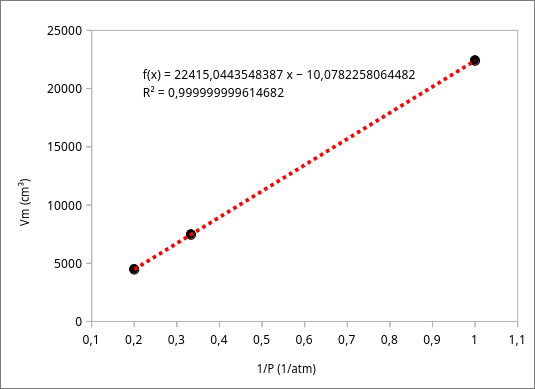
\includegraphics[width=.35\linewidth]{images/geo1.png}
        \caption{Regressão Linear de \(V_m\) em função de \( 1/P \) }
        \label{reggeo}
    \end{figure}
    Pela equação da reta dada pela regressão linear, obtemos o valor de \( RT \)
    e, então, determinamos R
    \begin{align*}
        R &= \frac{22415 \ \unit{cm^3.atm.mol^{-1}} }{273K} && (\text{Note o uso
        de 5 A.S.})\\
        &= 82,106 \ \unit{cm^3.atm.mol^{-1}.K^{-1}}
    \end{align*}
    Note que esse valor está desalinhado com o valor de referência em 0,05\%, que pode estar atrelado a erros experimentais.

\end{rsl}
